\documentclass{beamer}

\usepackage{beamerthemesplit}
\usepackage{tikz-uml}
%\usetheme{}

\title{Kolejka Projekt}
\subtitle{UML-Diagramm - Erster Entwurf}
\author{Gruppe A}
\date{\today}

\begin{document}
\maketitle
\frame{\tableofcontents[currentsection]}


\section{Überblick - UML-Diagramme}
\begin{frame}
	\frametitle{Klassenbeziehungen - Überblick}
    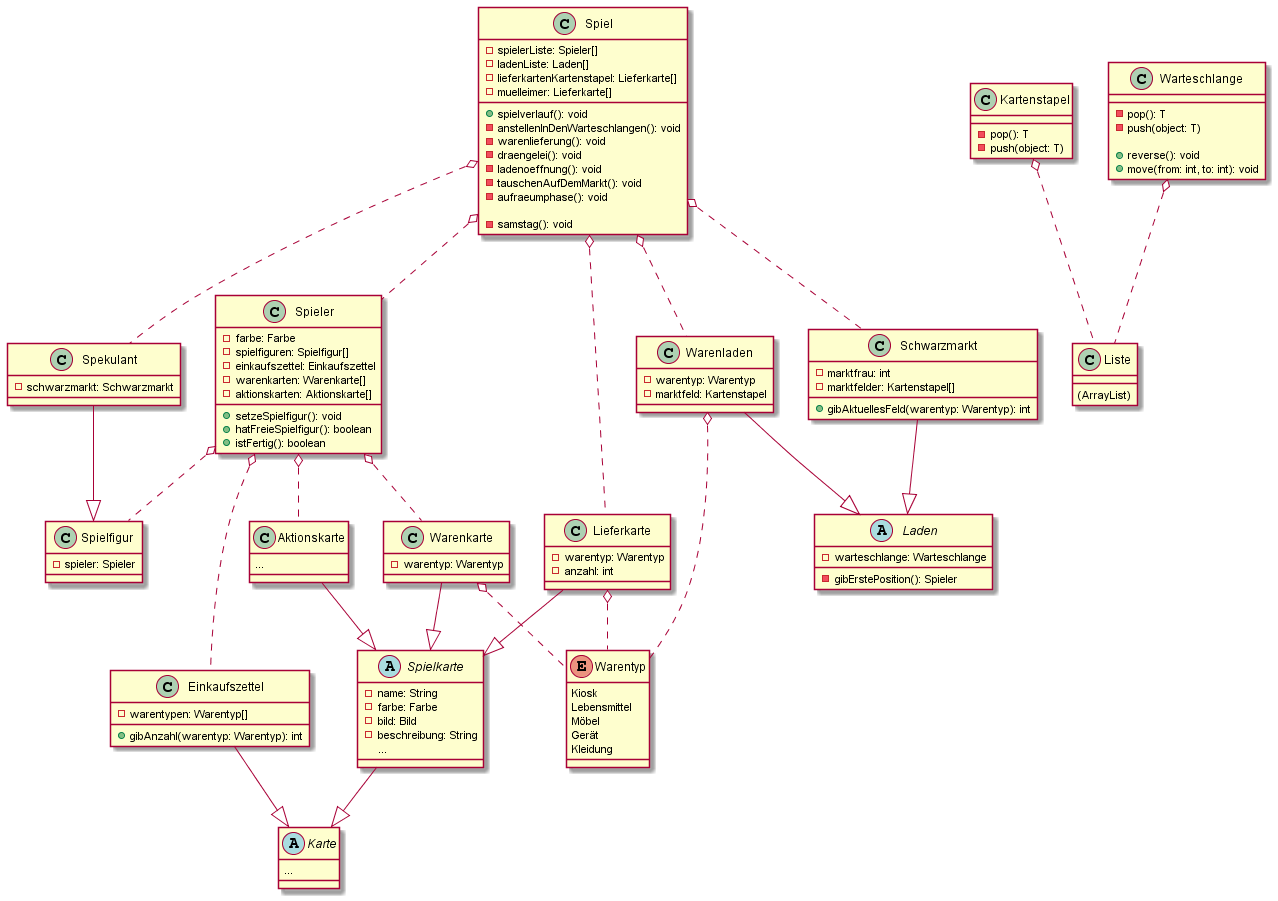
\includegraphics[height=0.85\textheight]{../../diagrams/out/architecture_overview/architecture_overview.png}
\end{frame}


\begin{frame}
	\frametitle{Klassenbeziehungen - Überblick - Umlet}
    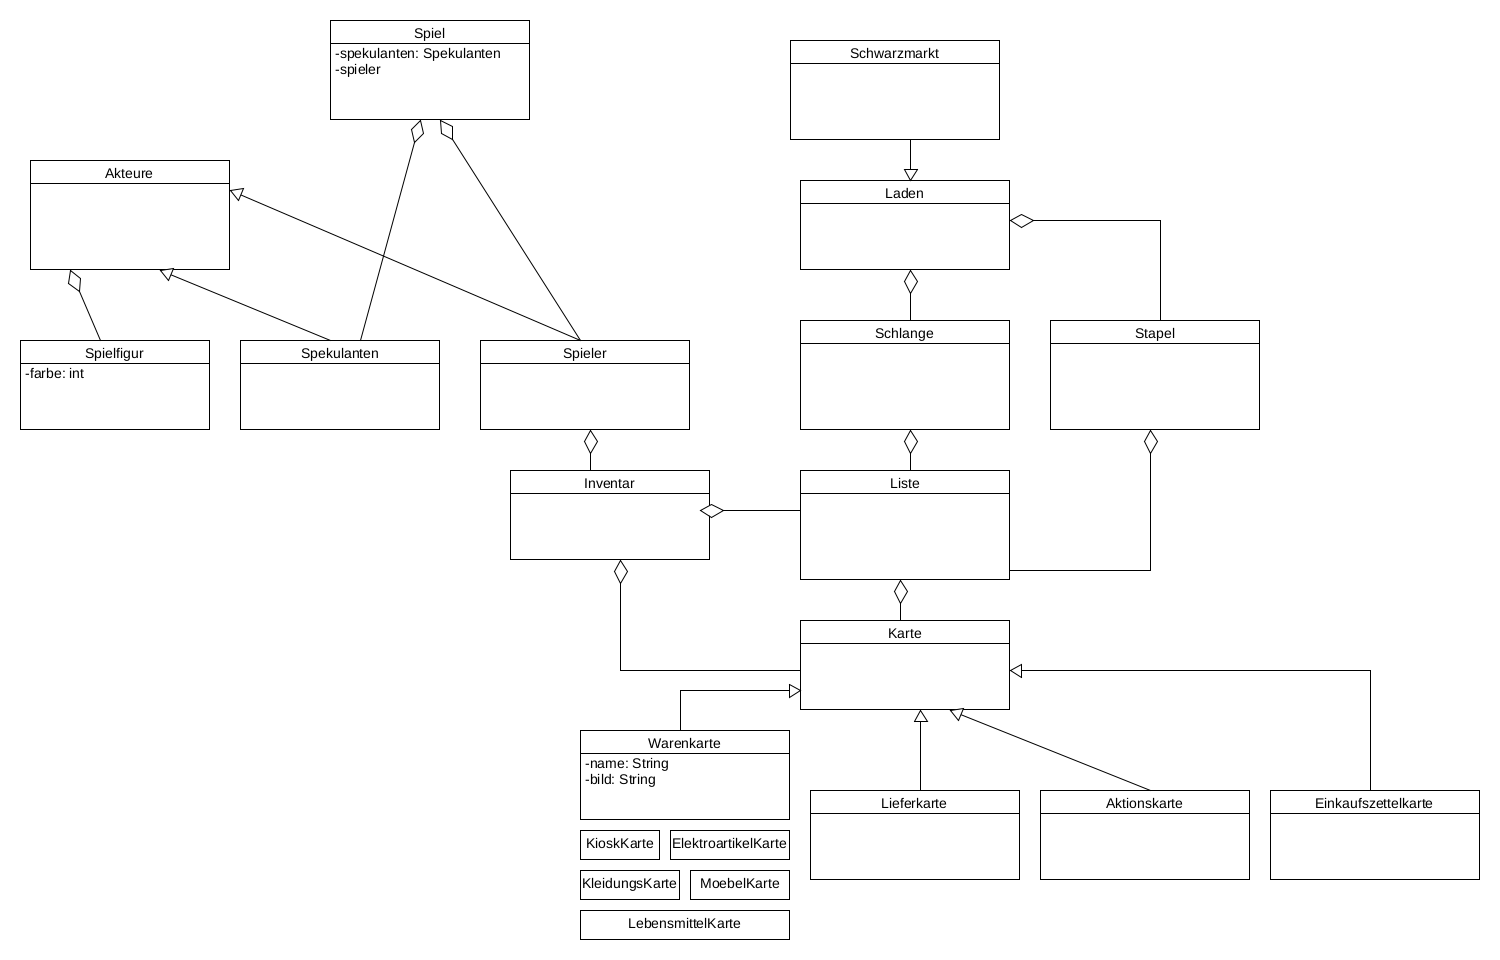
\includegraphics[height=0.8\textheight]{../../diagrams/umlet/kolejka_uml_26_04_2021.png}
\end{frame}


\begin{frame}
	\frametitle{Klassen}
	\begin{center}		
		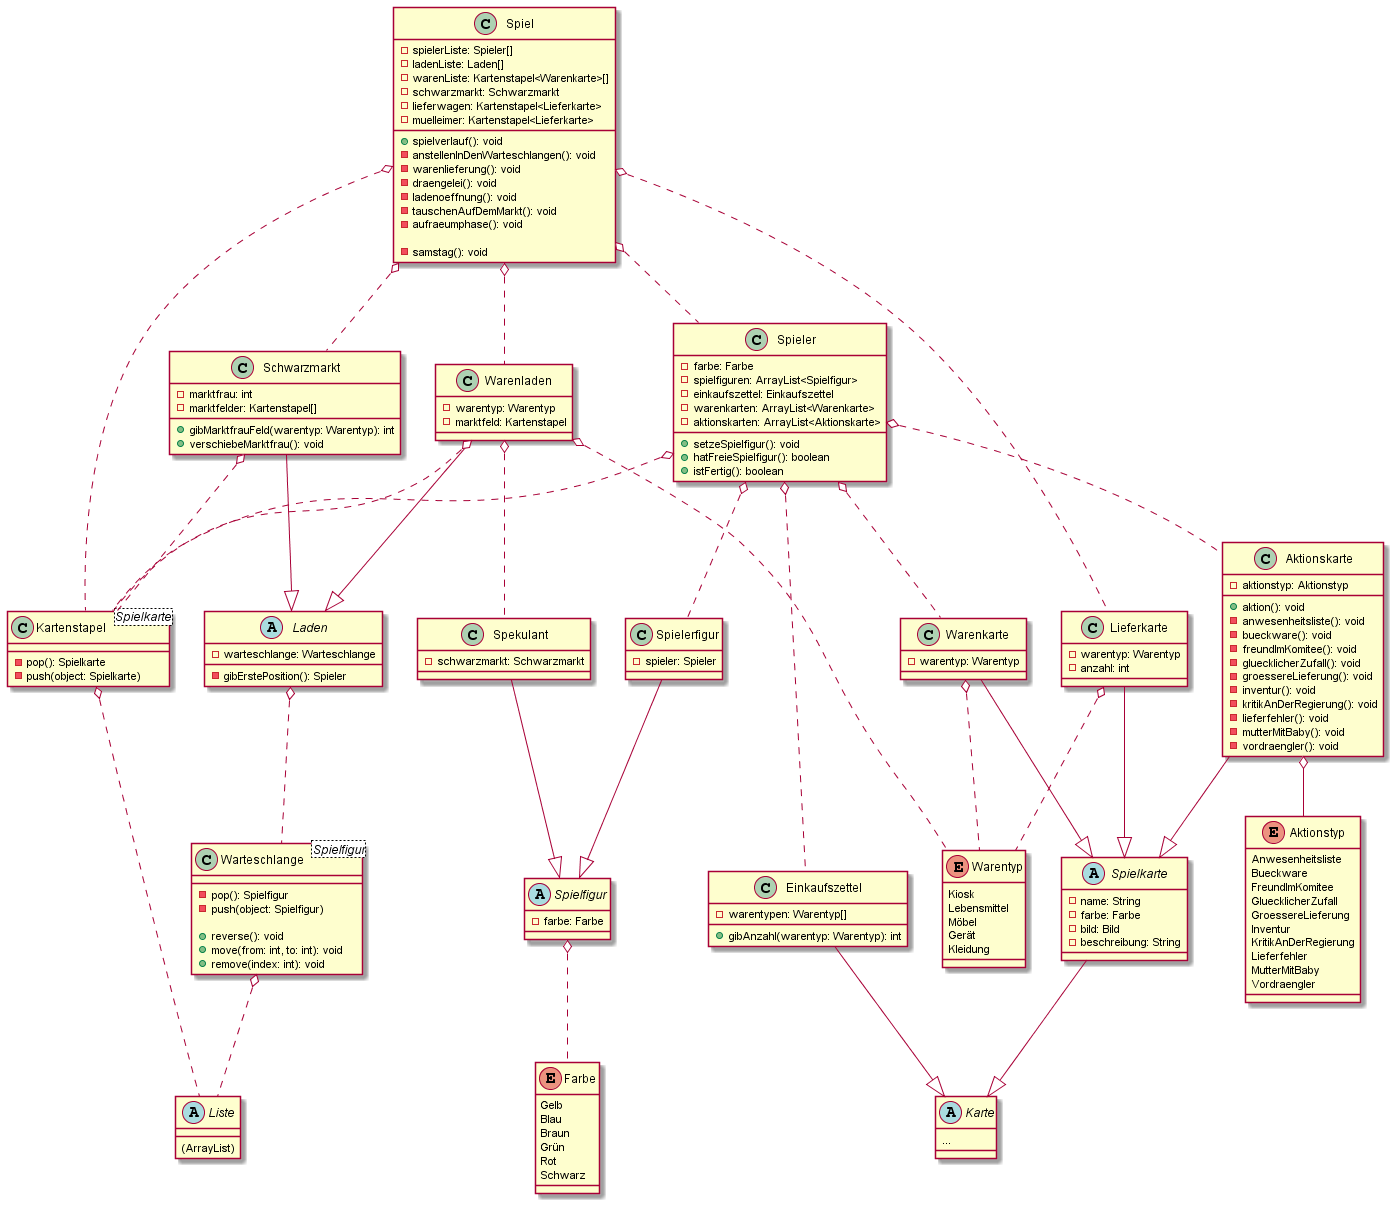
\includegraphics[width=1\textheight]{../../diagrams/out/classes/classes.png}
	\end{center}
\end{frame}

\section{Spiel und Spieler}
\begin{frame}
    \frametitle{Spiel}
    \begin{center}
        \begin{tikzpicture}
            \umlclass{Spiel}{
                -spielerListe:Spieler[]\\
                -ladenListe:Laden[]\\
                -warenListe:Kartenstapel$<$Warenkarte$>$[]\\
                -schwarzmarkt:Schwarzmarkt\\
                -lieferwagen:Kartenstapel$<$Lieferkarte$>$\\
                -muelleimer:Kartenstapel$<$Lieferkarte$>$\\ 
            }{
                +spielverlauf():void\\
                -anstellenInDenWarteschlangen():void\\  
                -warenlieferung():void\\
                -draengelei():void\\
                -ladenoeffnung():void\\
                -tauschenAufDemMarkt():void\\
                -aufraeumphase():void\\
                -samstag():void\\
            }
        \end{tikzpicture}
    \end{center}
\end{frame}

\begin{frame}
    \frametitle{Spieler}
    \begin{center}
        \begin{tikzpicture}
            \umlclass{Spieler}{
                -farbe:Farbe\\
                -spielfiguren:ArrayList$<$Spielfigur$>$\\
                -einkaufszettel:Einkaufszettel\\
                -warenkarten:ArrayList$<$Warenkarte$>$\\
                -aktionskarten:ArrayList$<$Aktionskarte$>$\\
            }{
                +setzeSpielfigur():void\\
                +hatFreieSpielfigur():boolean\\
                +istFertig():boolean\\
            }
        \end{tikzpicture}
    \end{center}
\end{frame}

\section{Läden}

\begin{frame}
    \frametitle{Schwarzmarkt}
    \begin{center}
        \begin{tikzpicture}
            \umlclass{Schwarzmarkt}{
                -marktfrau:int\\
                -marktfelder:Kartenstapel[]\\
            }{
                +gibMarktfrauFeld(warentyp: Warentyp):int\\
                +verschiebeMarktfrau():void
            }
        \end{tikzpicture}
    \end{center}
\end{frame}

\begin{frame}
    \frametitle{Warenladen}
    \begin{center}
        \begin{tikzpicture}
            \umlclass{Warenladen}{
                -warentyp:Warentyp\\
                -marktfeld:Kartenstapel\\
            }{
            }
        \end{tikzpicture}
    \end{center}
\end{frame}

\begin{frame}
    \frametitle{Laden}
    \begin{center}
        \begin{tikzpicture}
            \umlclass{Laden}{
                -warteschlange:Warteschlange\\
            }{
                +gibErstePosition():Spieler !Problematisch\\ 
            }
        \end{tikzpicture}
    \end{center}
\end{frame}

\section{Listen - Warteschlange und Kartenstapel}

\begin{frame}
    \frametitle{Liste}
    \begin{center}
        \begin{tikzpicture}
            \umlclass{Liste}{
                \#arrayList:ArrayList\\
            }{
                +toArray():Object[]\\
                +gib():Object\\
            }
        \end{tikzpicture}
    \end{center}
\end{frame}

\begin{frame}
    \frametitle{Warteschlange}
    \begin{center}
        \begin{tikzpicture}
            \umlclass{Warteschlange}{
            }{
                +anstellen():Spielfigur\\
                +entferneErsten(f:Spielfigur)\\
                +entferne(index:int):Spielfigur\\
                +umgekehrt():void\\
                +bewege(von:int,zu:int):void\\
                +tausche(i$1$:int,i$2$:int):void\\
            }
        \end{tikzpicture}
    \end{center}
\end{frame}

\begin{frame}
    \frametitle{Kartenstapel}
    \begin{center}
        \begin{tikzpicture}
            \umlclass{Kartenstapel}{
            }{
                +pop():Spielkarte\\
                +push(object:Spielkarte)\\
            }
        \end{tikzpicture}
    \end{center}
\end{frame}


\end{document}
